\chapter{Проектирование ПО для статического анализа кода системы компьютерной верстки TeX}

Необходимость создания специализированного программного обеспечения обусловлена необходимостью в оптимизации процесса проверки нормкотроля документов посредством человеческих усилий. За время наблюдения за процессом проверки работ на нормконтроль были замечены следующие моменты:

\begin{enumerate}
    \item каждый человек проверяет определенные моменты в силу своих знаний;
    \item каждый человек имеет разную длительность проверки;
    \item каждый человек может ошибаться в моментах проверки или же их пропускать.
\end{enumerate}

Конечным продуктом проверки является \guillemotleftудостоверение\guillemotright\verb| |о ее прохождении. Ввиду выше перечисленных моментов можно отметить, что у разных документов могут остаться различные ошибки и неточности, пропущенные или не проверенные конкретным человеком. Таким образом на представление общественности попадает недоделанный документ различной степени ошибочности, что является грубым нарушением правил нормконтроля и допуска к сдаче работы.

Разработанная программа позволит за короткое время проанализировать документ и предоставить информацию о неверном оформлении на основе заранее заданного шаблона и ожидаемых характеристик.

\section{Создание файла конфигурационных характеристик}

Ввиду того, что у каждого отдельно взятого учреждения или организации могут быть свои дополнительные правила по оформлению документов, наложенные или замещающие условно-общепринятые нормы, необходимо составить некоторый текстовый файл, который должен отображать требуемые для проверки характеристики. Данный файл должен создаваться отдельно под каждый различный тип оформления.

Файл должен иметь расширение \verb|.json| являющееся популярным и удобным для создания конфигурационных файлов. Рассмотрим каждую характеристику возможную конфигурационном файле. Если характеристики не обозначено в файле, то для нее применяется стандартное значение.

    Ссылки. Объект \verb|links| в файле содержит ключи относящиеся к настройке проверки ссылок конкретных элементов. Ключи описывают зарезервированные названия объектов среди, которых: \verb|figure|, \verb|equations|, \verb|table|, \verb|listings|, \verb|text|. Данные названия относятся к соответствующим аргументам команды \verb|\begin|: фигура, уравнение, таблица, листинг, а так же ссылки не выделенные в отдельный элемент. Ключ \verb|equations| (Листинг \ref{ls:01}) представляет собой внутреннюю структуру содержащую ключ \verb|position| принимающее в качестве значения массив содержащие резервированные слова \verb|before|, \verb|after|, которые означают возможность нахождение ссылки на элемент \verb|до| и \verb|после| нахождения данного элемента в тексте. Значение ключа \verb|caption| означает необходимость проверки на соответствие значения стоящего до ссылки текста, определяющее смысловое назначение ссылки на элемент. Ключ \verb|name| определяет необходимое имя для идентификации типов объектов ссылки. Ключ \verb|referToEverything| определяет необходимость ссылаться на каждый определенный элемент в тексте. 
    
    \begin{lstlisting}[caption = {Пример конфигурации ссылок}, label={ls:01}]
    "links" : {
      "equations": {
         "position" : ["before", "after"],  
         "caption" : ["Уравнение ", "уравнение "],
         "name" : "eq",
         "referToEverything" : true
      }
   }
    \end{lstlisting}

    Количество слов в названиях. Для того, чтобы давать наиболее полное представление о материале, находящемся в главах, параграфах и пунктах необходимо использовать распространённые предложения. Для отслеживания данного правила существует характеристика \verb|lengthOfNames|. Рассмотрим ключи и значения на примере Листинг . Ключи \verb|chapter|, \verb|section|, \verb|subsection|, \verb|caption| соответствуют смысловым определениям: глава, параграф, пункт, подпись. Каждый из ключей представляет собой структуру. Такие структуры содержат ключи \verb|minLength| и \verb|minWordLength|, соответственно означающие минимальное допустимое количество слов в названии и минимальную допустимую длину засчитываемого слова.  
    
     \begin{lstlisting}[caption = {Пример конфигурации названий}, label={ls:02}]
    "lengthOfNames":{
      "chapter" : {
         "minLength" : 3,
         "minWordLength" : 3
      },
      "section" : {
         "minLength" : 4
      },
      "subsection" : {
         "minLength" : 3
      },
      "caption":{
         "minLength" : 3
      }
   }
    \end{lstlisting}

    Списки. Характеристика \verb|lists| определяет форматирование и использования списков и их объектов.  Рассмотрим ключи и значения на примере Листинг \ref{ls:03}. Ключи, представляющие собой структуры соответствуют названиям списков. Опишем ключи и их смысловые значения структур характеристики \verb|lists|. Ключ \verb|itemOptions| определяется массивом значений возможных для использования в опциях команды \verb|\item|, в случае значения \verb|null| запрещается использование опций у данной команды. Ключ \verb|itemFormatting| представляет структуру, содержащую массивы символов, рассмотрим их подробнее. Массив значений ключа \verb|firstLetter| определяет возможность использования заглавных букв при значении \verb|A| как начальной после команды \verb|\item|, и аналогично использования строчных букв в случае значения \verb|a|. Ключ \verb|endLetter| определяет массив значений символов, один из которых должен быть в конце описываемого \verb|item|. Ключ \verb|lastStringEndLetter| определяет массив значений символов, один из которых должен быть в конце описываемого последнего \verb|item| списка. Значение ключа \verb|enableAnotherLists| определяет возможность использования в документе иных типов списков, кроме описанных. 
    \begin{lstlisting}[caption = {Пример конфигурации списков},label={ls:04}]
    "lists" :{
      "enumerate": {
         "itemOptions" : [null],
         "itemFormatting" :{
            "firstLetter" : ["A","a"],
            "endLetter" : [";"],
            "lastStringEndLetter" : ["."]
         }
      },
      "enableAnotherLists" : false   
   }
    \end{lstlisting}

    Ссылки на литературные источники. Данная характеристика описывается структурой \verb|biblioLinks| (Листитнг \ref{ls:04}). Структура отвечает за настройку форматирования и проверки ссылок на список литературы, описанный в файле с расширением \verb|.bib| и вызываемых по номеру в виде аргумента с помощью команды \verb|\cite|. Она содержит ключи с названиями  \verb|referBeforeSentenceEnd| и \verb|referToEverything|, соответственно означающие необходимость размещения ссылок до конца предложения, и необходимость использовать в тексте все ссылки на описанные литературные источники.
    
    \begin{lstlisting}[caption = {Пример конфигурации ссылок на литературные источники}, label={ls:04}]
    "biblioLinks" :{
          "referBeforeIndentStart" : true,
          "referToEverything" : true
       },
     \end{lstlisting}   

     Общее форматирование. Характеристика \verb|generalTextFormatting| содержит в себе смысловые ключи, которые не подходят для иных структур или представляют собой элементарную проверку. В качестве таких ключей выделяются \verb|useDashInsteadOfHyphen| означающий необходимость использовать тире вместо десисов между стоящих слов разделенных табуляцией и \verb|useGuillemotInsteadQuotationMarks| определяющий использования форматированных кавычек вместо обычных (Листинг \ref{ls:05}).

        \begin{lstlisting}[caption = {Пример общей конфигурации форматирования документа}, label={ls:05}]
     "generalTextFormatting" :{
      "useDashInsteadOfHyphen" : true,
      "useGuillemotInsteadQuotationMarks" : true
   }
     \end{lstlisting}   

\section{Подготовка файлов к статическому анализу}

Для начала проведения статического анализа, необходимо указать путь до архива с файлами расширения \verb|.tex| и иных файлов относящихся к документу, а так же путь до файла с расширением \verb|.json|, который будет является файлом характеристик. 

После запуска программы и указания путей проводится валидация файла характеристик на предмет корректности данных, ключей и значений. Успешная валидация позволяет перейти к следующему этапу работы программы -- формирование единого файла для удобного анализа. Данная операция включает в себя нахождение среди файлов такого, что содержит команды \verb|\begin{document}...\end{document}|. В случае ошибки поиска пользователю должны выдаться инстукции по корректировки файлов, чтобы создать необходимую структуру и повторно запустить программу.

Нахождение команд  \verb|\begin{document}...\end{document}| позволяет однозначно найти точку входа и выхода программы, тем самым определяя, что весь текст и команды относящиеся к компиляции документа находятся между началом и концом \guillemotleftблока\guillemotright  \verb| document|. Зная данную информацию, программа переходит по относительным путям к файлам и копирует содержимое в общий файл в порядке, заданном в исходном файле. 

По итогу текущего этапа программа имеет информацию о необходимых к проверке характеристиках и полный текст документа. 

\section{Синтаксического и лексический анализ общего файла}

Данный этап позволяет получить структуру файла, и занести необходимые команды и текст в отдельные объекты, которые понадобятся в дальнейших операциях программы. 

Чтобы получить оперируемую структуру исходного файла, необходимо выполнить поиск по соответствию шаблону. В качестве шаблона выступают строки, в виде регулярных выражений, для поиска отдельных команд и вхождений в тексте. Таким образом в тексте выявляются команды, определяются их аргументы и опции следующего вида \verb|\command_name{args}[options]|. Найденное вхождение создает объект куда, записывается информация о команде:

\begin{enumerate}
    \item название;
    \item тип;
    \item аргументы;
    \item опции;
    \item длина полной строки;
    \item начальный и конечный номера символов.
\end{enumerate}

В дальнейшем по списку данных объектов будет производится поиск и выявление проблемных мест функциями анализа.

\section{Выполнение статического анализа характеристик}
    Рассмотрим порядок выполнения действий по проверки характеристик файла конфигурации.
    
    \verb|links|. Проверка корректности документа относительно данной характеристики происходит в несколько этапов. Нахождение среди списка команд команды \verb|\begin{arg}|, где в качестве \verb|arg| представляется одно из ключевых слов. Нахождение внутри блока команды \verb|\label| задающее название ссылки на элемент. Проверка ее значения на соответствие в ключем \verb|name|. В случае успешного соответствия, определяется полный вид ссылки и происходит поиск команды \verb|\ref{}| с аргументом являющимся искомой ссылкой. В случае ненахождения ссылки и значения ключа \verb|\referToEverything| равняется true выдается сообщение о необходимости создать ссылку. Далее, проверяется относительные позиции ссылки и элемента на соответствие с ключом \verb|position|. Находится начало ссылки, и минуя знаки табуляции определяется ближайшее стоящее слово и происходит проверка с массивом допустимых значений. 

    \verb|lengthOfNames|. Функция, запускающая проверку данной характеристики поэтапно проверяет каждую структурный ключ описанный в характеристике, где начальным этапом обозначается нахождение соответствующей ключу команды, и затем выполнение проверки длины аргумента относительно количества слов и букв в словах.

    \verb|lists|. Выполняемая функция проводит поиск среди списка команд команды \verb|\begin{arg}|, где в качестве \verb|arg| представляется одно из ключевых слов. Внутри блочного элемента находятся команды \verb|\item| и производится соответствие опций данной команды со массивом значений ключа \verb|itemOptions|. Далее происходит поиск первого и последнего нетабулативного символа с проверкой на соответствие начертанию относительно массива значений ключа \verb|firstLetter| и \verb|endLetter| соответственно, и \verb|lastStringEndLetter| в случае последнего значащего символа последнего элемента \verb|\item|.

     \verb|biblioLinks|. Для проверки характеристики осуществляется выделение номеров из файла библиографии в отдельный список, значения которых последовательно будут использоваться в качестве аргументов в процессе поиска команды \verb|\cite|. Если значение ключа \verb|referToEverything| равняется \verb|true|, то в случае ненахождения соответствующей ссылки в тексте сообщение об ошибке создается относительно текстовой позиции номера литературного источника в файле библиографии. После нахождения команды, проверяется наличие символов отличных от абзацной или подобной табуляции после найденной команды для проверки по ключу \verb|referBeforeIndentStart|. 

    \verb|generalTextFormatting|. Каждый ключ данной характеристики можно считать, как отдельную характеристику ввиду необходимости запуска соответствующей функции для каждого отдельно взятого ключа. Ключ \verb|useDashInsteadOfHyphen| -- происходит поиск символа \guillemotleftдефис\guillemotright и проверяется наличие символов табуляции по обе стороны от дефиса. Если такая проверка оказалась успешной, то создается сообщение о необходимости замены символа на \guillemotleftтире\guillemotright. Ключ \verb|useGuillemotInsteadQuotationMarks| -- происходит поиск символа \guillemotleftдвойные кавычки\guillemotright\verb| | и создается сообщение о необходимости замены его на команды \verb|\guillemotleft| и  \verb|\guillemotright| относительно позиции кавычек к оборачиваемой словесной конструкции.
    
    В случае любых ошибочных проверок создается запись об ошибке с текстовыми координатами в виде строки и символа в строке с соответствующим сообщением об ошибке.

 Все сообщение об ошибках с соответствующими характеристикам данными формируют единый файл, с которым человек, запустивший программу обязан ознакомится и приложить усилия по исправлению найденных проблем.

\section{Общая схема работы программы}

    Описав отдельно различные аспекты программы составим общую схему работы программы (Рисунок \ref{fig:3}). В качестве входных данных поступают полный архив с файлами \verb|.tex| и иными необходимыми файлами и конфигурационный файл в формате \verb|.json| Значения и ключи  конфигурационного файла записываются в соответствующие значения программы для определение списка необходимых для выполнения функций. Архив же находит исходный файл, из которого формируется общий файл для проведение синтаксического и лексического анализа для выделения команд с их названием аргументами, опциями, и иной информацией. После анализа последовательно выполняется каждая функция и в случае необходимости вносит данные в переменную со всеми встреченными ошибками. По окончанию работы последней функции, переменная записывается в файл, и он сохраняется на компьютере пользователя.

   \begin{figure}[!h]
        \center
        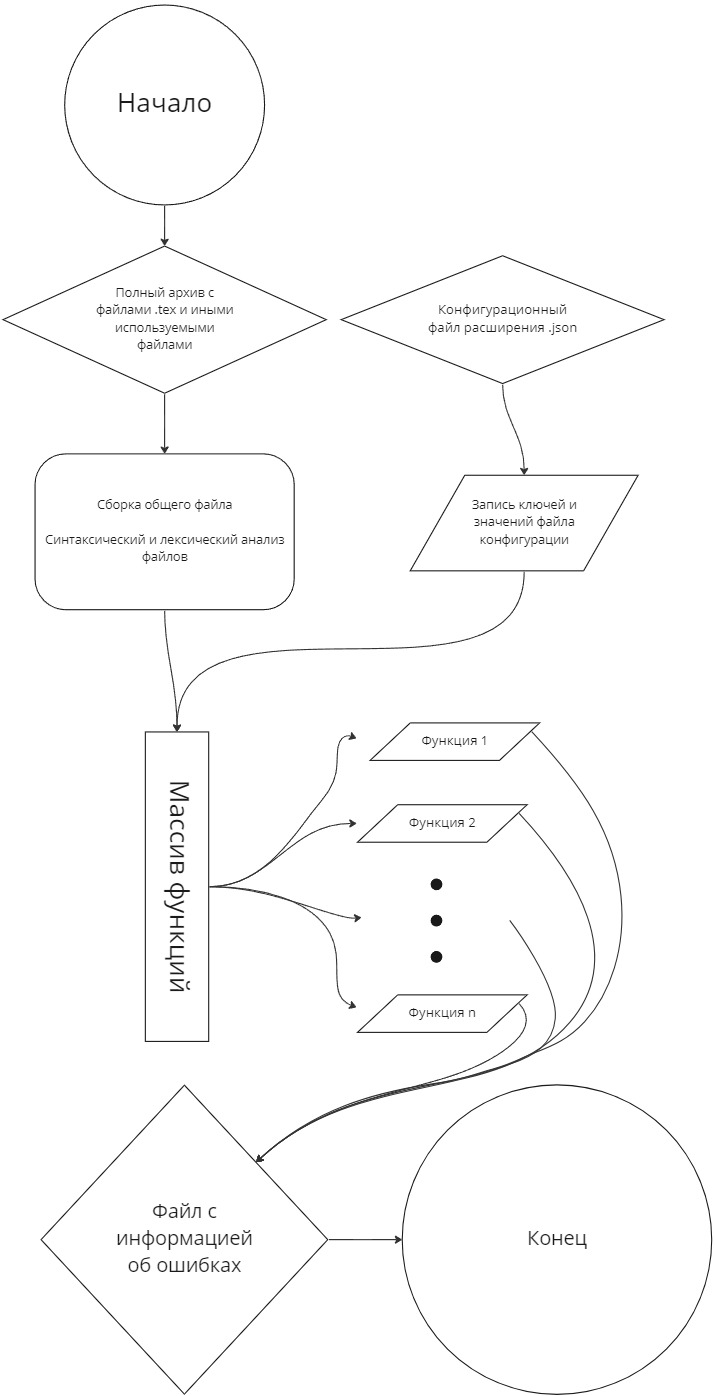
\includegraphics[width=12cm]{Images/WorkToGo.png}
        \caption{Общая схема работы программы}
        \label{fig:3}
    \end{figure}
